\section{Modeling Scattered/Reflected Spectra (Two–Stream Approximation)$^\ddagger$}

When scattering and reflection are present, flux–based two–stream approximations are commonly used. Here we proceed as follows.

For a plane–parallel atmosphere, the radiative transfer equation is
\begin{align}
\mu \frac{d \Ilam}{d \tau} = \Ilam - \Jlam .
\label{eq:radtrantau_start}
\end{align}

First, since extinction includes both absorption and scattering, we write
\begin{align}
\kappa_\nu = \mu_a + \mu_s ,
\label{eq:extsaa}
\end{align}
where $\mu_a$ is the true absorption coefficient and $\mu_s$ the scattering coefficient.

For the emission, let us include thermal emission (C) and scattering of upward radiation from below (D). Cases E–H correspond to external illumination (e.g., starlight) and are needed when modeling reflected stellar light, but we will not consider them here. In this setup the emission coefficient is the sum of thermal and scattering contributions,
\begin{align}
\eta_\nu = \mu_a B_\nu + \mu_s \frac{1}{4 \pi} \int d \Omega \, \mathcal{P}(\Omega)\, \Ilam ,
\label{eq:emisaa}
\end{align}
where, in the first term on the right–hand side, neglecting scattering would recover absorption = emission (Kirchhoff's law). Thus we assume local thermodynamic equilibrium (LTE), under which the emission spectrum is Planckian by detailed balance.\footnote{This assumption can break down in the upper atmosphere—for Earth, above roughly the mesosphere.} The second term represents scattering; $\mathcal{P}(\Omega)$ encodes the angular dependence of the scattering phase function (e.g., for scattering by thin clouds).

The source function is then
\begin{align}
\Jlam = \frac{\eta_\nu}{\kappa_\nu} = (1-\omega_0) B_\nu + \frac{\omega_0}{4 \pi} \int d \Omega \, \mathcal{P}(\Omega)\, \Ilam ,
\label{eq:sourcef}
\end{align}
where
\begin{align}
\omega_0 \equiv \frac{\mu_s}{\mu_a + \mu_s}
\label{eq:sia}
\end{align}
is the single–scattering albedo.

It is convenient to describe the angular distribution of the specific intensity using its angular moments, i.e., integrals over solid angle weighted by powers of $\mu$. Define the global (full–sphere) angular average
\begin{align}
\label{eq:all_int}
\langle \mathcal{F} \rangle \equiv \frac{1}{4\pi} \int d\Omega \, \mathcal{P}(\Omega)\, \mathcal{F}
= \frac{1}{4\pi} \int d\phi \int_{-1}^{1} d\mu \, \mathcal{P}(\Omega)\, \mathcal{F} .
\end{align}
We denote the zeroth, first, and second moments by
\begin{align}
\Jl &\equiv \langle \Ilam \rangle ,\\
\Hl &\equiv \langle \mu \Ilam \rangle ,\\
\Kl &\equiv \langle \mu^2 \Ilam \rangle .
\end{align}

Using the zeroth moment, the source function can be written compactly as
\begin{align}
\Jlam = \frac{\eta_\nu}{\kappa_\nu} = \omega_0 J_\nu + (1-\omega_0) B_\nu .
\label{eq:sourcef}
\end{align}

Accordingly, the radiative transfer equation becomes
\begin{align}
\label{eq:rtbasic}
\mu \frac{d \Ilam(\Omega)}{d \tau}
= \Ilam(\Omega) - \omega_0 J_\nu - (1-\omega_0) B_\nu .
\end{align}

In the two–stream approximation, we split quantities into an upward (outgoing) flux and a downward (incoming) flux. We integrate over the upper hemisphere (US) and the lower hemisphere (LS). Keeping the moment equations in mind, define the hemispheric angular–average operator for an arbitrary function $\mathcal{F}$ by
\begin{align}
\label{eq:us_int}
  \langle \mathcal{F} \rangle_\mathrm{US}
  &\equiv \frac{1}{4\pi} \int_{\mathrm{US}} d\Omega \, \mathcal{P}(\Omega)\, \mathcal{F}
   = \frac{1}{4\pi} \int d\phi \int_{0}^{1} d\mu \, \mathcal{P}(\Omega)\, \mathcal{F},\\
\label{eq:ls_int}
  \langle \mathcal{F} \rangle_\mathrm{LS}
  &\equiv -\,\frac{1}{4\pi} \int_{\mathrm{LS}} d\Omega \, \mathcal{P}(\Omega)\, \mathcal{F}
   = \frac{1}{4\pi} \int d\phi \int_{0}^{-1} d\mu \, \mathcal{P}(\Omega)\, \mathcal{F}.
\end{align}
In the two–stream convention we insert the minus sign in the LS definition so that downward quantities are positive; note, therefore, that
\begin{align}
\langle \mathcal{F} \rangle = \langle \mathcal{F} \rangle_\mathrm{US} - \langle \mathcal{F} \rangle_\mathrm{LS}.
\end{align}

The upward–emitted flux from the atmosphere is obtained by weighting the intensity with the upward directional cosine and integrating over the upper hemisphere:
\begin{align}
F^+ = \int_{\mathrm{US}} d\Omega \, \mu \, \mathcal{P}(\Omega)\, \Ilam(\Omega)
= 4\pi \,\big\langle \mu \, \Ilam(\Omega) \big\rangle_\mathrm{US},
\end{align}
where we may write $\Ilam(\Omega) = \Ilam(\mu)$.

If the scattering is isotropic, $\mathcal{P}(\Omega)=1$, and the azimuthal dependence of the intensity can be neglected, this reduces to
\begin{align}
F^+ = 2\pi \int_{0}^{1} d\mu \, \mu \, \Ilam(\mu).
\end{align}

\subsection*{Direct solution without scattering and the transmission function}

When there is no scattering ($\omega_0=0$), and if we neglect the azimuthal dependence so that the intensity depends only on $\mu$ (i.e., $\Ilam(\Omega)=\Ilam(\mu)$), equation (\ref{eq:rtbasic}) can be solved analytically for $\Ilam(\mu)$ by multiplying both sides by $e^{-\tau/\mu}$ and integrating. Namely,
\begin{align}
\label{eq:analypuabs}
\frac{d}{d \tau} \left( \Ilam(\tau,\mu) e^{-\tau/\mu} \right) = - \frac{B_\nu \bigl(T(\tau)\bigr)}{\mu} \, e^{-\tau/\mu} .
\end{align}
Consider a single atmospheric layer as in Fig.~\ref{fig:layer1}, and denote the intensity at the bottom and top of the layer by $\Ilam(\tau_1,\mu)=\Ilams_1(\mu)$ and $\Ilam(\tau_2,\mu)=\Ilams_2(\mu)$, respectively. From (\ref{eq:analypuabs}) we obtain
\begin{align}
\Ilams_1 (\mu) = \Ilams_2 (\mu) \, e^{-\Delta \tau/\mu} + \frac{1}{\mu} \int_{\tau_1}^{\tau_2} d \tau \, \Blam \bigl(T(\tau)\bigr) \, e^{- (\tau - \tau_1)/\mu} ,
\end{align}
where $\Delta \tau=\tau_2-\tau_1$. Multiplying by $2\pi\mu$ and integrating over the upper hemisphere gives the upward flux from the top of the layer $F_{+,1}$:
\begin{align}
\label{eq:onelayer}
F_{+,1} &= 2 \pi \int_{0}^1 d\mu \, \mu \, \Ilams_1 (\mu) \\
&= 2 \pi \int_{0}^1 d\mu \, \Ilams_2 (\mu) \, \mu \, e^{-\Delta \tau/\mu} \nonumber \\
&\quad +  \int_{\tau_1}^{\tau_2} d \tau \, \pi \, \Blam \bigl(T(\tau)\bigr) \, \mathcal{G} (\tau - \tau_1) ,\\
\mathcal{G} (\tau) &\equiv 2 \int_{0}^1 d\mu \, e^{-\tau/\mu} .
\end{align}
This expression is fairly transparent: the upward flux emerging from the top consists of the upward intensity incident from below, attenuated by $e^{-\Delta \tau/\mu}$ and integrated over the upper hemisphere with the $\mu$ weight, plus the layer’s own thermal emission, each contribution being attenuated on its way to the top by the factor $\mathcal{G}(x)$ (see Fig.~\ref{fig:transrt}). In particular, if we take the top of the atmosphere as the upper boundary (i.e., $\tau_1=0$) and neglect radiation from below (set $\Ilam_2=0$), equation (\ref{eq:onelayer}) reduces to
\begin{align}
\label{eq:onelayer_}
F_{+,1} = \int_{0}^{\infty} d \tau \, \pi \, \Blam \bigl(T(\tau)\bigr) \, \mathcal{G} (\tau) .
\end{align}

\begin{figure}[htb]
\begin{center}
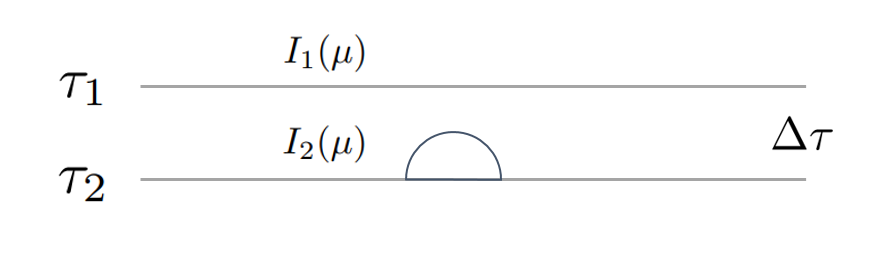
\includegraphics[width=\linewidth]{fig/layer1.PNG}
\caption{\label{fig:layer1}}
\end{center}
\end{figure}

\begin{figure}[htb]
\begin{center}
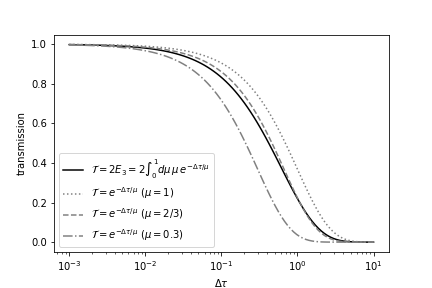
\includegraphics[width=\linewidth]{fig/transrt.PNG}
\caption{Transmission function for the pure–absorption case.\label{fig:transrt}}
%exojax/examples/tutorial/pure\, absorption\, rt.ipynb
\end{center}
\end{figure}



\subsection*{Approximation via Moment Closure}

(e.g., see Meadow \& Weaver 80 \cite{1980JAtS...37..630M} and Toon et al. 1989 \cite{1989JGR....9416287T}). First, for the upper hemisphere (US) and lower hemisphere (LS), define the zeroth moment (mean intensity)
\begin{align}
\Jl_+ &\equiv \langle\Ilam \rangle_\mathrm{US} \\
\Jl_- &\equiv \langle\Ilam \rangle_\mathrm{LS} 
\end{align}
and the first moment,
\begin{align}
\Hl_+ &\equiv \langle\mu \Ilam \rangle_\mathrm{US} \\
\Hl_- &\equiv \langle\mu \Ilam \rangle_\mathrm{LS} 
\end{align}
while the upward and downward fluxes are
\begin{align}
F^+ &= 4 \pi H_+ \\
F_- &= 4 \pi H_-
\end{align}
respectively.

The radiative transfer equations are
\begin{align}
\label{eq:ratvvx}
 &\frac{d  }{d \tau} \langle\mu  \Ilam (\Omega) \rangle_\mathrm{US} \nonumber \\
 &=  \langle \Ilam(\Omega) \rangle_\mathrm{US}  - \omega_0 \langle \mu  \rangle_\mathrm{US} J_\nu - (1-\omega_0) \langle\mu \rangle_\mathrm{US} \Blam \\
 \label{eq:ratvv2x}
 &\frac{d  }{d \tau} \langle\mu^2  \Ilam (\Omega) \rangle_\mathrm{LS} \nonumber \\
 &=  \langle\mu \Ilam(\Omega) \rangle_\mathrm{LS} - \omega_0 \langle \mu \rangle_\mathrm{LS} J_\nu  - (1-\omega_0)\langle\mu \rangle_\mathrm{LS} \Blam  
 \end{align}
Hence, since $\langle \mu \rangle_\mathrm{US}=-\langle \mu \rangle_\mathrm{LS}=1/2$,
\begin{align}
\label{eq:ratvv}
 \frac{d  }{d \tau} \langle\mu  \Ilam (\Omega) \rangle_\mathrm{US}  &=  \langle\Ilam(\Omega) \rangle_\mathrm{US} - \frac{\omega_0}{2} J_\nu  - \frac{(1-\omega_0)}{2} \Blam  \\
 \label{eq:ratvv2}
 \frac{d  }{d \tau} \langle\mu  \Ilam (\Omega) \rangle_\mathrm{LS}  &=  \langle \Ilam(\Omega) \rangle_\mathrm{LS}  + \frac{\omega_0}{2} J_\nu - \frac{(1-\omega_0)}{2} \Blam  
 \end{align}

Here, using $\Jl = \Jl_+ - \Jl_-$ and adopting the closure relations
\begin{align}
\eta_+ &= \Jl_+/\Hl_+ \\
\eta_- &= - \Jl_-/\Hl_- 
\end{align}
we obtain
\begin{align}
\label{eq:ratvvA}
\dot{\Hl}_+ &= \eta_+ \left( 1 - \frac{\omega_0}{2}\right) \Hl_+ - \frac{ \omega_0}{2}  \Hl_- - \frac{(1-\omega_0)}{2} \Blam  \\
 \label{eq:ratvv2A}
 \dot{\Hl}_- &= \frac{\eta_+ \omega_0}{2} \Hl_+ -  \eta_- \left( 1 - \frac{ \omega_0}{2}\right) \Hl_- + \frac{(1-\omega_0)}{2} \Blam
 \end{align}
or, equivalently,
\begin{align}
\label{eq:ratvvA}
\dot{F}_+ &= \eta_+ \left( 1 - \frac{\omega_0}{2}\right) F^+ -  \frac{\eta_- \omega_0}{2}  F_- - 2 \pi (1-\omega_0) \Blam  \\
 \label{eq:ratvv2A}
 \dot{F}_- &= \frac{\eta_+ \omega_0}{2} F^+ -  \eta_- \left( 1 - \frac{ \omega_0}{2}\right) F_- + 2 \pi (1-\omega_0) \Blam
 \end{align}

If we assume the closure relations for the upper and lower hemispheres have the same form, then $\eta_+ = \eta_- \equiv \eta$, and
\begin{align}
\label{eq:ratvvAaVV}
\dot{F}_+ (\tau) &= \gamma_1 F^+ (\tau) - \gamma_2  F_- (\tau) - 2 \pi (1-\omega_0) \Blam  (\tau) \\
 \label{eq:ratvv2A}
 \dot{F}_- (\tau) &=  \gamma_2 F^+ (\tau) - \gamma_1 F_- (\tau) + 2 \pi (1-\omega_0) \Blam (\tau)
 \end{align}
where we have set
\begin{align}
\gamma_1 &\equiv\eta \left( 1 - \frac{\omega_0}{2}\right) \\
\gamma_2 &\equiv\frac{\eta \, \omega_0}{2}
\end{align}
so that $\gamma_1+\gamma_2=\eta$ and $\gamma_1-\gamma_2=\eta (1-\omega_0)$.

Equations (\ref{eq:ratvvAaVV},\ref{eq:ratvv2A}) form a system of first-order coupled differential equations, i.e., a homogeneous system augmented by $\tau$-dependent terms originating from $\Blam(\tau)$. Therefore, by Taylor-expanding $\Blam(\tau)$ and approximating it with a truncated finite polynomial, one can obtain solutions.

Choosing $\gamma_1 = 2 - \omega_0$ and $\gamma_2 = \omega_0$ recovers the hemispheric-mean approximation with asymmetry parameter $g=0$ \cite{1989JGR....9416287T}. To solve Eqs.~(\ref{eq:ratvvAaVV}) and (\ref{eq:ratvv2A}), define new quantities $\Fsum \equiv F^+ + F_-$ and $\Fnet \equiv F^+ - F_-$; rewriting yields
\begin{align}
%\dFnet &= \eta (1 - \omega_0) \Fsum - 4 \pi (1- \omega_0) \Bl\\
%\dFsum &= \eta \Fnet
\dFnet &= (\gamma_1 - \gamma_2) \Fsum - 4 \pi (1- \omega_0) \Bl\\
\dFsum &=  (\gamma_1 + \gamma_2)  \Fnet,
\end{align}
from which the second-order equation
\begin{align}
%\ddFsum - \eta^2 (1 - \omega_0) \Fsum + 4 \pi (1-\omega_0) \Bl = 0.
\ddFsum - (\gamma_1^2 - \gamma_2^2)  \Fsum + 4 \pi (1-\omega_0) (\gamma_1 + \gamma_2) \Bl = 0.
\end{align}
is obtained.

Let us retain only the first-order term in the Taylor expansion of $\Bl$ with respect to $\tau$ \cite{1989JGR....9416287T} \cite{heng2017exoplanetary}:
\begin{align}
\Bl \approx B_0 + \dot{B} (\tau - \tau_0).
\end{align}
In this case, the solutions are
\begin{align}
\Fsum &= c_1 e^{\lambda \tau} + c_2 e^{-\lambda \tau} +\frac{ 4 \pi (1-\omega_0)}{\gamma_1 - \gamma_2} \Bl \\
\Fnet &= c_1 \delta e^{\lambda \tau} - c_2 \delta e^{-\lambda \tau} +\frac{ 4 \pi (1-\omega_0)}{\gamma_1^2 - \gamma_2^2} \dBl,
\end{align}
%where $\lambda \equiv \eta (1-\omega_0)^{1/2}$. 
where
\begin{align}
\lambda &\equiv\sqrt{\gamma_1^2-\gamma_2^2} \\
\delta &\equiv\sqrt{\frac{\gamma_1 - \gamma_2}{\gamma_1 + \gamma_2}}.
\end{align}

Substituting the above back into $F^+$ and $F_-$ gives
\begin{align}
F^+ (\tau) &= c_1 \zeta_+ e^{\lambda \tau} + c_2 \zeta_- e^{-\lambda \tau} + \pi \mathcal{B}_+ (\tau)  \\
F^- (\tau) &= c_1 \zeta_- e^{\lambda \tau} + c_2 \zeta_+ e^{-\lambda \tau} + \pi \mathcal{B}_- (\tau)
\end{align}
where
\begin{align}
 \mathcal{B}_\pm(\tau) &\equiv\frac{ 2 (1-\omega_0)}{\gamma_1 - \gamma_2} \left( \Bl(\tau) \pm \frac{1}{\gamma_1 + \gamma_2} \dBl (\tau) \right) \\
 \zeta_\pm &\equiv\frac{1}{2} (1 \pm \delta).
\end{align}
The $\zeta_\pm$ are called the coupling coefficients \cite{heng2017exoplanetary}. \\
\subsection*{Solving Radiative Transfer in an Atmospheric Layer Model}

Up to this point we have derived the hemispheric-mean two-stream approximation, but the solutions for the upward and downward streams in the Toon89-type two-stream approximation can be written in the same form:
\begin{align}
\label{eq:2stream_1}
F^+ (\tau) &= c_1 \zeta^+ e^{\lambda \tau} + c_2 \zeta^- e^{-\lambda \tau} + \pi \mathcal{B}^+ (\tau)  \\
\label{eq:2stream_2}
F^- (\tau) &= c_1 \zeta^- e^{\lambda \tau} + c_2 \zeta^+ e^{-\lambda \tau} + \pi \mathcal{B}^- (\tau)
\end{align}
Here, $\zeta^\pm$ are called the coupling coefficients. Notably, the two-stream approximation in the spherical harmonics (SH) method takes the same form. We therefore consider solving radiative transfer for an atmospheric layer model starting from equations of this form.

% How \omega and g relate to \gamma_1, \gamma_2, and \zeta
In the above equations, $\zeta^{\pm}$ and $\lambda$ are related to the coefficients $\gamma_1$ and $\gamma_2$ of the differential equations for $F^{\pm}$ as
\begin{align}
    \zeta^\pm &= \frac{1}{2} \left( 1 \pm \sqrt{\frac{\gamma_1 - \gamma_2}{\gamma_1 + \gamma_2}} \right)\\
    \lambda &= \sqrt{\gamma_1^2 - \gamma_2^2},
\end{align}
The coefficients $\gamma_1$ and $\gamma_2$ are determined by the single-scattering albedo $\omega$ and the asymmetry parameter $g$, and this relationship depends on the choice of moment closure \cite{1989JGR....9416287T}. When using the hemispheric mean,
the relations $\gamma_1 = 2 - \omega (1 + g)$ and $\gamma_2 = \omega (1 - g)$ hold. The reduced source function is expressed as
\begin{align}
\mathcal{B}^\pm (\tau) = 
    \frac{ 2 (1-\omega)}{\gamma_1 - \gamma_2} \left( \Bl(\tau) \pm \frac{1}{\gamma_1 + \gamma_2} \dBl (\tau) \right).
\end{align}
In the above expression, the second term can be neglected for an isothermal layer.

Equations (\ref{eq:2stream_1}, \ref{eq:2stream_2}) can be written as
\begin{align}
    \Fv(\tau) = Q(\tau) \xv + \pi \Bv (\tau)
\end{align}
where $\Fv (\tau) = (F^+ (\tau), F^-(\tau))^\top$, $\Bv (\tau) = (\mathcal{B}^+ (\tau), \mathcal{B}^- (\tau))^\top$, $\xv \equiv (c_1, c_2)^\top$, and
\begin{align}
    Q(\tau) = \left(
\begin{array}{cc}
\zeta^+ e^{\lambda \tau} & \zeta^- e^{-\lambda \tau}  \\
\zeta^- e^{\lambda \tau} & \zeta^+ e^{-\lambda \tau}  \\
\end{array}
\right)
\end{align}

%\subsubsection*{Standard linear form for a uniform-layer model}
Next, consider an $N$-layer model with optical thickness differences $\Delta \tau_n$, and define the optical depth at the top of layer $n$ as $\tau = \tau_n = \sum_{i=0}^{n-1} \Delta \tau_i$ ($n \ge 1$) with $\tau_0 = 0$.

Consider the $n$-th layer:
\begin{align}
\label{eq:Fv1}
    \Fv (\tau_n) &= Q_n(\tau_n) \xv_n + \pi \Bv_n (\tau_n) = \Fv_n\\
\label{eq:Fv2}
    \Fv (\tau_n+\Delta \tau_n) &= Q_n(\tau_n + \Delta \tau_n) \xv_n + \pi \Bv_n (\tau_n + \Delta \tau_n) \nonumber \\
    &= \Fv_{n+1}
\end{align}
Here $Q_n$ is defined as $Q(\tau)$ for the $n$-th layer. Thus, once the internal parameters $\zeta^\pm_n$ and $\lambda_n$ of the $n$-th layer are set,
\begin{align}
    Q_n(\tau) = \left(
\begin{array}{cc}
\zeta^+_n e^{\lambda_n \tau} & \zeta^-_n e^{-\lambda_n \tau}  \\
\zeta^-_n e^{\lambda_n \tau} & \zeta^+_n e^{-\lambda_n \tau}  \\
\end{array}
\right).
\end{align}

From (\ref{eq:Fv1}) and (\ref{eq:Fv2}), we obtain the linear recursive form
\begin{align}
    \label{eq:rtstandard}
    \Fv_{n+1} &= \mathcal{G} (\Delta \tau_n) \Fv_n + \pi \Gv_n,
\end{align}
where
\begin{align}
   \Gv_n \equiv \Bv_n (\tau_n + \Delta \tau_n) - \mathcal{G} (\Delta \tau_n) \Bv_n (\tau_n)  
\end{align}
and $\Gv_n = (G_n^+, G_n^-)^\top$.
We define the transfer function as
\begin{align}
\label{eq:transfer_matrix}
\mathcal{G} (\Delta \tau_n) &\equiv Q(\tau_n + \Delta \tau_n) Q^{-1}(\tau_n) \\
&=  Q_n(\tau_n)
 \left(
\begin{array}{cc}
e^{\lambda_n \Delta \tau_n}  & 0  \\
0 & e^{-\lambda_n \Delta \tau_n}  \\
\end{array}
\right) Q_n^{-1}(\tau_n) \nonumber \\
\end{align}
This is the eigendecomposition $ \mathcal{G} (\Delta \tau_n) \qv_i = \lambda^\prime_i \qv_i$, where $\qv_i$ denotes the $i$-th column vector of $Q_n(\tau_n)$. Therefore, the vectors $\qv_i$ can be normalized; in particular, $\qv_1$ can be normalized by $e^{\lambda_n \tau_n}$ and $\qv_2$ by $e^{-\lambda_n \tau_n}$. By defining
\begin{align}
    Z_n \equiv Q_n(0) = \left(
\begin{array}{cc}
\zeta^+_n  & \zeta^-_n  \\
\zeta^-_n & \zeta^+_n  \\
\end{array}
\right),
\end{align}
the above can be rewritten as
\begin{align}
\label{eq:transfer_matrix2}
&\,\mathcal{G} (\Delta \tau_n) = 
 Z_n
 \left(
\begin{array}{cc}
e^{\lambda_n \Delta \tau_n}  & 0  \\
0 & e^{-\lambda_n \Delta \tau_n}  \\
\end{array}
\right) Z_n^{-1} \\
\label{eq:gzero}
&= \frac{1}{{\zeta^+_n}^2 - {\zeta^-_n}^2} \nonumber \\
&\times \left(
\begin{array}{cc}
  {\zeta^+_n}^2 e^{t_n} - {\zeta^-_n}^2 e^{-t_n} & \,  - \zeta^+_n \zeta^-_n (e^{t_n} - e^{-t_n}) \\
\zeta^+_n \zeta^-_n (e^{t_n} - e^{-t_n})& \, {\zeta^+_n}^2 e^{-t_n} - {\zeta^-_n}^2 e^{t_n} \\
\end{array}
\right), \nonumber \\
\end{align}
where
\begin{align}
t_n \equiv \lambda_n \Delta \tau_n
\end{align}
is a function of $\Delta \tau_n$ but not of $\tau_n$.

For an isothermal layer, $\Bv_n (\tau_n) = \Bv_n (\tau_n + \Delta \tau) \equiv \mathcal{B}_n \uv$, with $\mathcal{B}_n = \mathcal{B}^+ (\tau_n) = \mathcal{B}^- (\tau_n)$, where $\uv$ is the unit vector $\uv \equiv (1,1)^\top$. The source vector $\Gv_n$ can then be simplified as
\begin{align}
\Gv_n &= \mathcal{B}_n (I - \mathcal{G} (\Delta \tau_n) ) \uv \\
&= \frac{\mathcal{B}_n}{\zeta_n^+ + \zeta_n^-} \left(
\begin{array}{c}
     \zeta_n^+ (1 - e^{t_n}) + \zeta_n^- (1 - e^{-t_n}) \\
    \zeta_n^+ (1 - e^{-t_n}) + \zeta_n^- (1 - e^{t_n})
\end{array}
\right)
\end{align}
where $I$ is the identity matrix.\\




\subsubsection*{Transfer within a Single Layer}

While the linear form (\ref{eq:rtstandard}) is mathematically concise, its physical meaning is not transparent. We therefore convert it to a form that represents the transport of radiation within a single layer.

From (\ref{eq:rtstandard}) we obtain
\begin{align}
    F^+_n = \Gaa^{-1} F^+_{n+1} - \Gaa^{-1} \Gab F^-_n -\Gaa^{-1} \pi G_n^+,
\end{align}
where $\mathcal{G}_{ij}$ denotes the $(i,j)$ component of $\mathcal{G}(\Delta \tau_n)$ with the index $n$ suppressed in the symbol. Substituting this into
$F^-_{n+1} = \Gba F^+_{n} + \Gbb F^-_n + \pi G_n^-$ yields
\begin{align}
F^-_{n+1} &= \Gba \Gaa^{-1} F^+_{n+1} + (\Gbb - \Gba \Gaa^{-1} \Gab) F^-_n \nonumber \\
&\quad + \pi G_n^- - \Gba \Gaa^{-1} \pi G_n^+ .
\end{align}

In the two-stream case, from (\ref{eq:gzero}) we have $\Gba = -\Gab$ and $\Gaa^{-1} = \Gbb - \Gba \Gaa^{-1} \Gab \equiv \mathcal{T}_n$ as well as $\Gba \Gaa^{-1} = - \Gaa^{-1} \Gab \equiv \mathcal{S}_n$. Accordingly, the radiative transfer within the $n$-th layer can be written as
\begin{align}
\label{eq:twosq1}
 F^+_n &= \mathcal{T}_n F^+_{n+1} + \mathcal{S}_n F^-_n - \mathcal{T}_n \pi G_n^+ \\
 \label{eq:twosq2}
 F^-_{n+1} &= \mathcal{T}_n F^-_{n} + \mathcal{S}_n F^+_{n+1} + \pi G_n^- - \mathcal{S}_n \pi G_n^+,
\end{align}
where
\begin{align}
\label{eq:transmission_onelayer}
 &\mathcal{T}_n \equiv 
 \frac{{{\zeta^+_n}}^2 -{{\zeta^-_n}}^2 }{{\zeta^+_n}^2  - (\zeta^-_n\mathsf{T}_n)^2 } \,\mathsf{T}_n \\
 \label{eq:scattering_onelayer}
&\mathcal{S}_n  \equiv 
\frac{\zeta^+_n \zeta^-_n }{{\zeta^+_n}^2  - (\zeta^-_n\mathsf{T}_n)^2 } \,(1-\mathsf{T}_n^2)
 \end{align}
can be interpreted as the transmittance between the bottom and top of the layer and the scattering of flux from the opposite direction, respectively\footnote{If we define the opaque (optically thick) limit of the scattering in (\ref{eq:scattering_onelayer}) as $S_\infty \equiv \zeta_-/\zeta_+$ for $\mathsf{T}_n=0$, then (\ref{eq:scattering_onelayer_}) can be rewritten in a form analogous to that used in the flux-adding treatment of \cite{2023PSJ.....4...10R}:
\begin{align}
\label{eq:scattering_onelayer_}
 \mathcal{T}_n = \frac{S_\infty \, ( 1 - e^{-2 \lambda_n \Delta \tau_n})}{1 - S_\infty^2  e^{-2 \lambda_n \Delta \tau_n} } .
 \end{align}
 For the hemispheric-mean case, we obtain
 \begin{align}
     S_\infty &= \frac{\sqrt{1-\omega g}-\sqrt{1-\omega}}{\sqrt{1-\omega g}+\sqrt{1-\omega}} \\
     \lambda_n &= 2 \sqrt{(1-\omega g)(1-\omega)}.
 \end{align}
 }. In the above expressions, following \cite{heng2017exoplanetary} we define the transmission function
 \begin{align}
 \label{eq:opacity_transfer}
 \mathsf{T}_n &\equiv e^{-\lambda_n \Delta \tau_n}.
\end{align} 
Note that (\ref{eq:twosq1}, \ref{eq:twosq2}) are essentially the same as the analytic two-stream expressions derived by \cite{heng2017exoplanetary}\footnote{Equation (3.58) of \cite{heng2017exoplanetary}. In our notation, $\lambda_n$ corresponds to $\mathcal{D}$ in \cite{heng2017exoplanetary}.}.

For an isothermal layer, (\ref{eq:twosq1}) and (\ref{eq:twosq2}) simplify to
\begin{align}
\label{eq:twosq1iso}
 F^+_n &= \mathcal{T}_n F^+_{n+1} + \mathcal{S}_n F^-_n + \pi \hat{\mathcal{B}}_n\\
 \label{eq:twosq2iso}
 F^-_{n+1} &= \mathcal{T}_n F^-_{n} + \mathcal{S}_n F^+_{n+1} + \pi \hat{\mathcal{B}}_n
\end{align}
where
\begin{align}
    \hat{\mathcal{B}}_n \equiv (1 - \mathcal{T}_n - \mathcal{S}_n) \mathcal{B}_n.
\end{align}

\subsection*{flux-adding treatment}\label{ss:flux-adding}

As a solution technique for the two-stream approximation including scattering, the flux-adding treatment \cite{2018JQSRT.211...78R,2023PSJ.....4...10R}, which utilizes a reflectance form, has been proposed. It is derived by analogy with the classical adding method. The flux-adding treatment assumes that, within a given layer, the upward flux can be expressed as the sum of the reflection of the downward flux and a source term from the layer:
\begin{align}
    \label{eq:fa1}
    F_n^+ &= \hat{R}_n^+ F_n^- + \hat{S}_n^+ \\
    \label{eq:fa2}
    F_n^- &= \hat{R}_n^- F_n^+ + \hat{S}_n^-.
\end{align}

Replacing $F_n^+$ in (\ref{eq:twosq1iso}) with (\ref{eq:fa1}) and multiplying by $\mathcal{T}_n$ yields
\begin{align}
    \mathcal{T}_n^2 F_{n+1}^+ = (\hat{R}_n^+ - \mathcal{S}_n) \mathcal{T}_n F_n^- + \mathcal{T}_n (\hat{S}_n^+ - \pi \hat{\mathcal{B}}_n).
\end{align}
Eliminating $F_n^-$ from the above using (\ref{eq:twosq2iso}) gives
\begin{align}
    \label{eq:recursive_fa}
    F_{n+1}^+ &= \frac{\hat{R}_n^+ - \mathcal{S}_n}{  \mathcal{T}_n^2 -\mathcal{S}_n^2 +  \mathcal{S}_n \hat{R}_n^+} F_{n+1}^- \nonumber \\
    &+ \frac{\hat{\mathcal{B}}_n(\mathcal{S}_n - \mathcal{T}_n- \hat{R}_n^+ ) + \mathcal{T}_n \hat{S}_n^+}{  \mathcal{T}_n^2 -\mathcal{S}_n^2 +  \mathcal{S}_n \hat{R}_n^+}.
\end{align}
Let the coefficient of the first term on the right-hand side be $\hat{R}_{n+1}^+$ and the second term be $\hat{S}_{n+1}^+$. This leads to the following recurrence relations:
\begin{align}
    \label{eq:fa_Rplus}
    \hat{R}_n^+ &= \mathcal{S}_n + \frac{\mathcal{T}_n^2 \hat{R}_{n+1}^+}{1-\mathcal{S}_n \hat{R}_{n+1}^+} \\
    \label{eq:fa_Splus}
    \hat{S}_n^+ &= \hat{\mathcal{B}}_n + \frac{\mathcal{T}_n (\hat{S}_{n+1} + \hat{\mathcal{B}}_n \hat{R}_{n+1}^+)}{1 - \mathcal{S}_n \hat{R}_{n+1}^+}.
\end{align}
In deriving (\ref{eq:fa_Splus}), (\ref{eq:fa_Rplus}) was used to eliminate $R_n^+$ from the second term in (\ref{eq:recursive_fa}).

Thus, assuming the reflectivity (i.e., albedo) at the lower boundary of the bottom layer ($n=N-1$), one can compute $\hat{R}^+_0$ and $\hat{S}^+_0$ and obtain the emergent flux at the top of the atmosphere as
\begin{align}
    F_0^+ = \hat{R}^+_0 F_\star + \hat{S}^+_0,
\end{align}
where $F_\star$ is the incident stellar flux.

Although $\hat{R}^-_n$ and $\hat{S}^-_n$ are not required to compute the emergent flux, they can also be derived. Replacing $n$ by $n-1$ in (\ref{eq:twosq2iso}), then using (\ref{eq:fa2}) to eliminate $F_n^-$, and further extracting $\mathcal{T}_{n-1} F_n^+$ by substituting $n \to n-1$ in (\ref{eq:twosq1iso}) and inserting it into the above, we obtain
\begin{align}
    \label{eq:recursive_fa2}
    F_{n-1}^- &= \frac{\hat{R}_n^- - \mathcal{S}_{n-1}}{  \mathcal{T}_{n-1}^2 -\mathcal{S}_{n-1}^2 +  \mathcal{S}_{n-1} \hat{R}_n^-} F_{n-1}^+ \nonumber \\
    &+ \frac{\hat{\mathcal{B}}_{n-1}(\mathcal{S}_{n-1} - \mathcal{T}_{n-1}- \hat{R}_n^- ) + \mathcal{T}_{n-1} \hat{S}_n^-}{  \mathcal{T}_{n-1}^2 -\mathcal{S}_{n-1}^2 +  \mathcal{S}_{n-1} \hat{R}_n^-}.
\end{align}
Defining the coefficient of the first term on the right-hand side as $\hat{R}_{n-1}^-$ and the second term as $\hat{S}_{n-1}^-$ yields the recurrences
\begin{align}
    \label{eq:fa_Rminus}
    \hat{R}_n^- &= \mathcal{S}_{n-1} + \frac{\mathcal{T}_{n-1}^2 \hat{R}_{n-1}^-}{1 - \mathcal{S}_{n-1} \hat{R}_{n-1}^-} \\
    \label{eq:fa_Sminus}
    \hat{S}_n^- &= \hat{\mathcal{B}}_{n-1} + \frac{\mathcal{T}_{n-1} (\hat{S}_{n-1} + \hat{\mathcal{B}}_{n-1} \hat{R}_{n-1}^-)}{1 - \mathcal{S}_{n-1} \hat{R}_{n-1}^-}.
\end{align}

Equations (\ref{eq:fa_Rplus}), (\ref{eq:fa_Splus}), (\ref{eq:fa_Rminus}), and (\ref{eq:fa_Sminus}) are essentially the same as Eqs. (7), (8), (4), and (5) of \cite{2018JQSRT.211...78R}.

As seen above, in the flux-adding treatment one can formulate and solve recurrence relations by including scattering as the sum of an effective reflection and a source term for each layer. Likewise, by including scattering as the sum of an effective transmission and a source term for each layer, alternative recurrences can be formulated. Although we have not yet identified a practical advantage of this method, it is a natural flux-based extension of pure absorption and is of theoretical interest.
